\documentclass[landscape,a0paper, fontscale=.285]{baposter}
\usepackage{graphics}
\usepackage{color}
\usepackage{multicol}
\usepackage{amsmath}
\usepackage{amssymb, wasysym}
\usepackage{lipsum}
\usepackage{graphicx}
\usepackage{enumitem}
\usepackage{listings}
\pdfcompresslevel=1

\begin{document}
\definecolor{myfavoritecolor}{rgb}{0.0 2.55 0}

%:Background image
\background{
      \begin{tikzpicture}[remember picture,overlay]%
      \draw (current page.center)+(-0em,-10em) node[anchor=center]
      {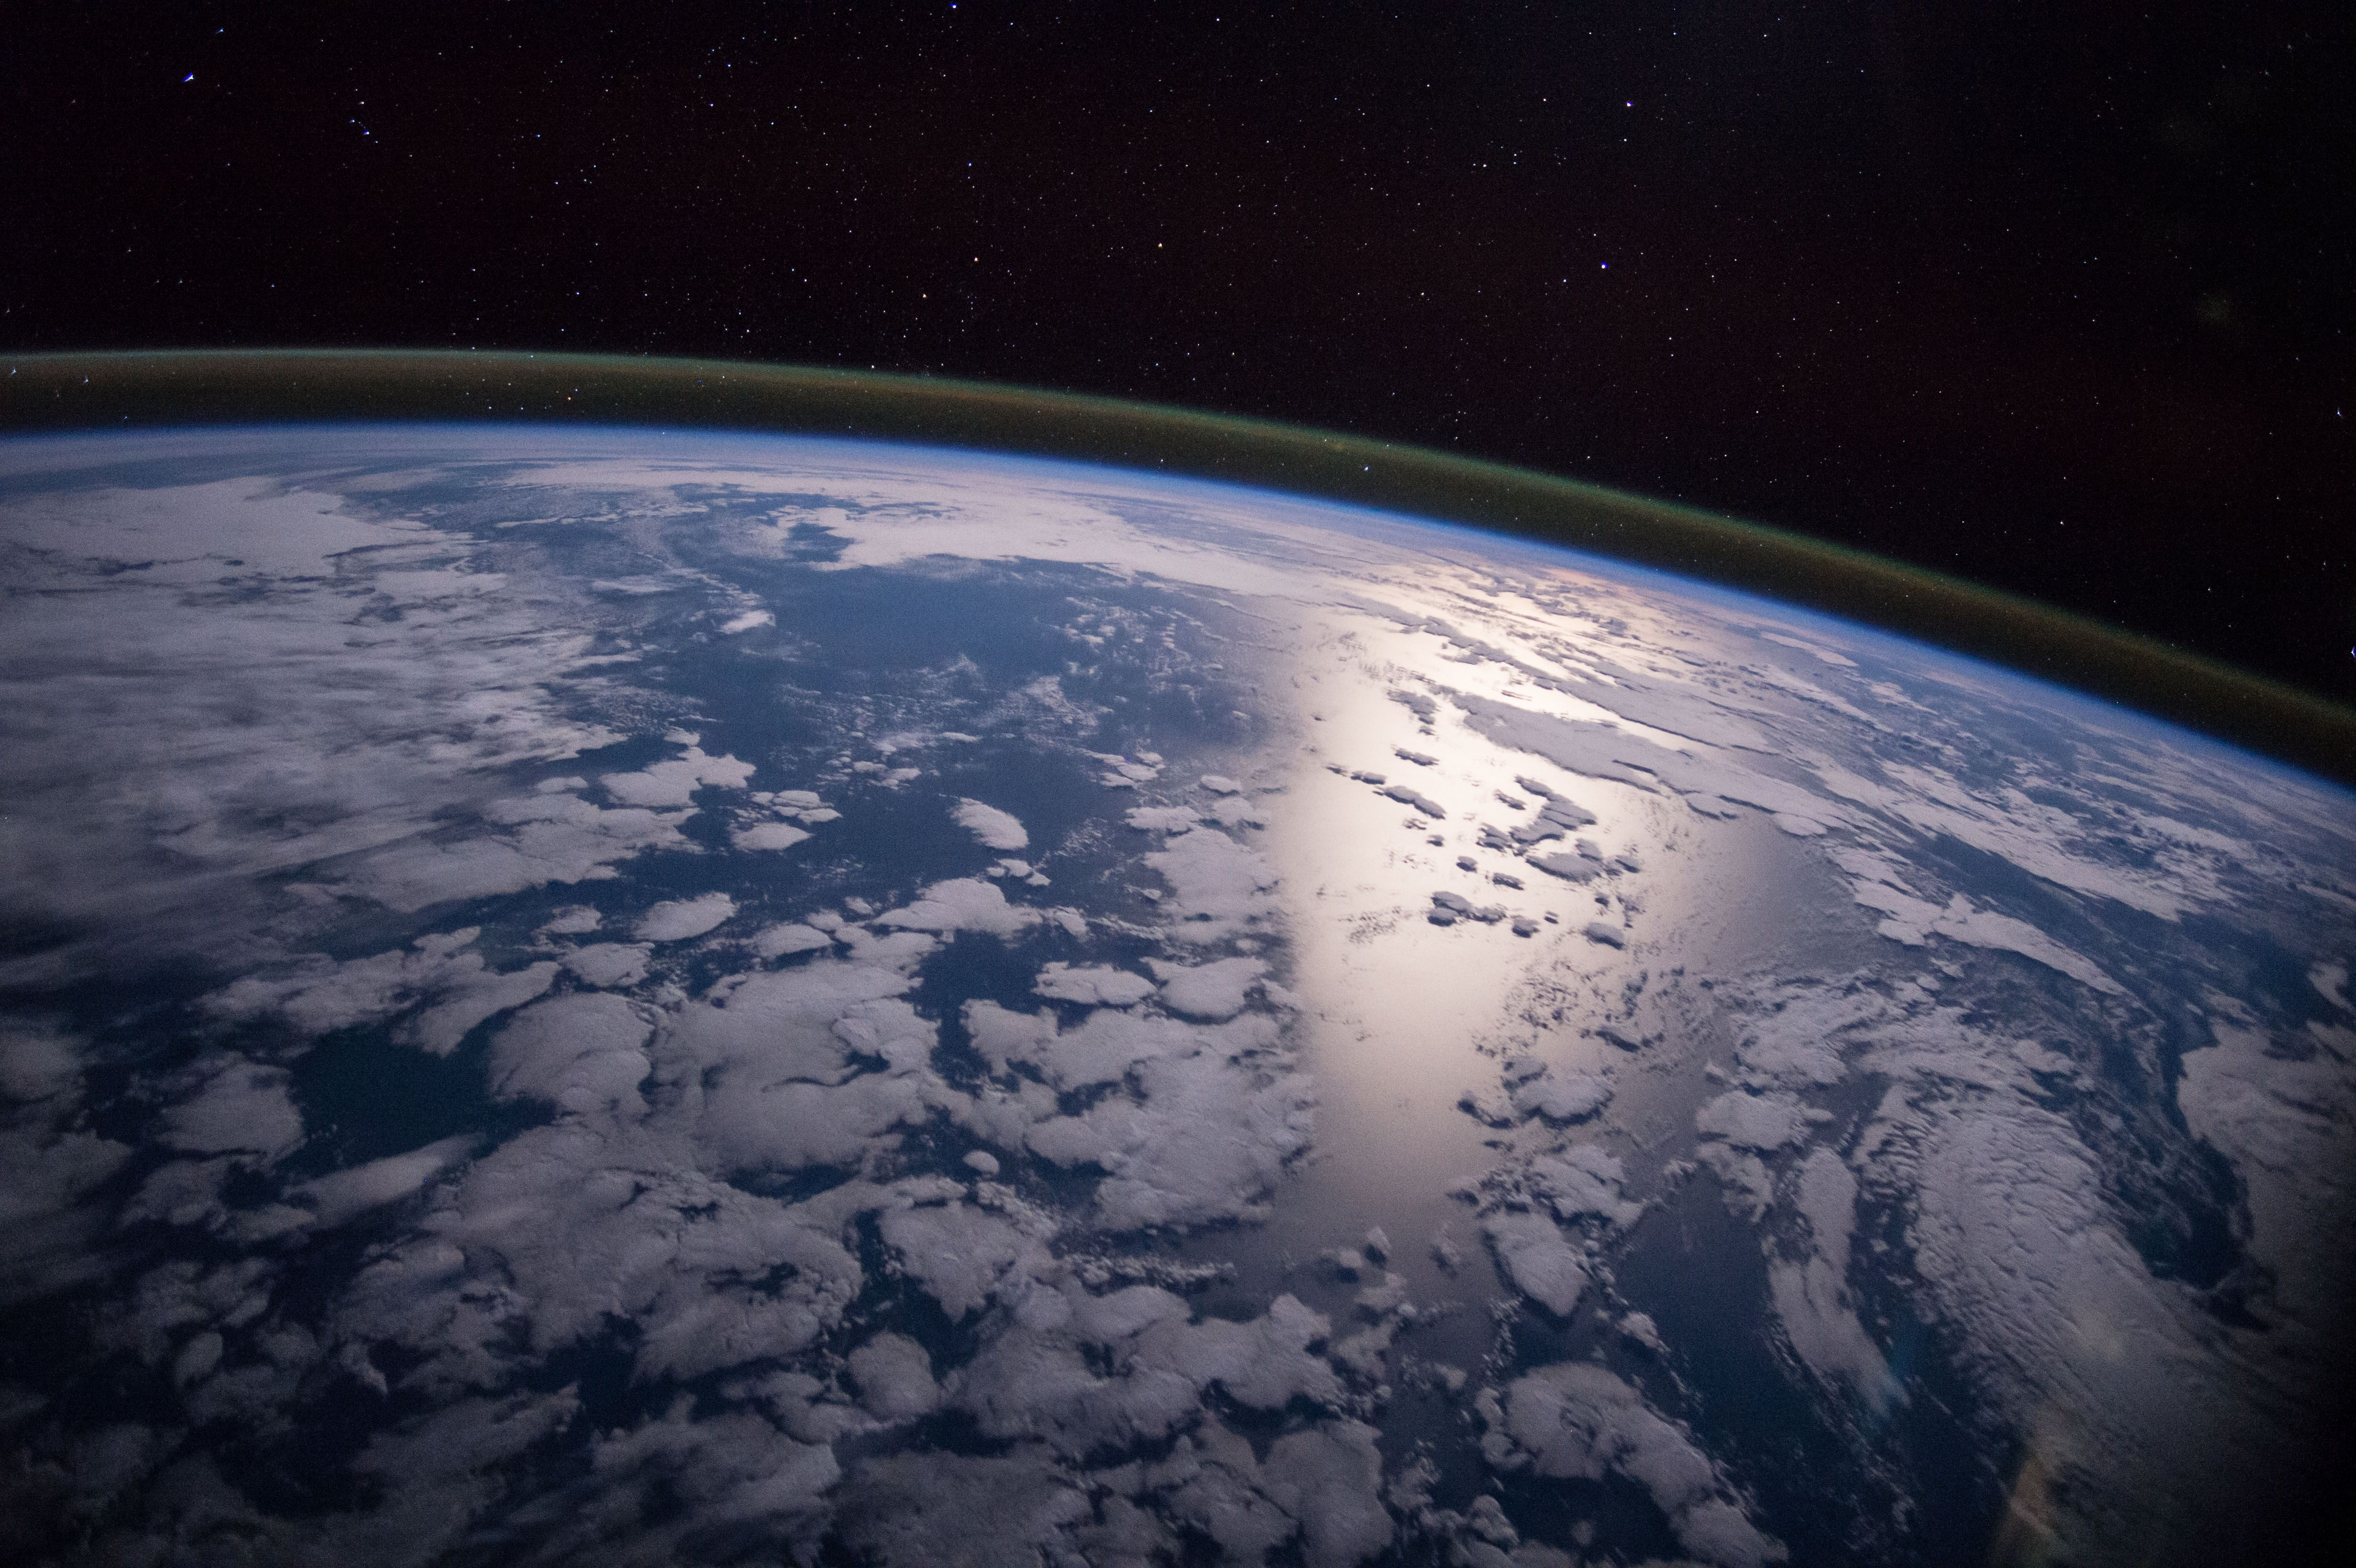
\includegraphics[width=1.41\textwidth]{images/background.jpg}};;
      \end{tikzpicture}%
      }

\begin{poster}
{%Keyword=value pairs
  % Color style
background = user,
 bgColorOne=white,
  bgColorTwo=red,
  borderColor=black,
  headerColorOne=black,
  headerColorTwo=gray,
  headerFontColor=white,
  boxColorOne=white,
  boxColorTwo=myfavoritecolor,
  % Format of textbox
  textborder=roundedleft,
  % Format of text header
  eyecatcher=true,
  headerborder=closed,
  headerheight=0.15\textheight,
  headershape=roundedright,
  headershade=shadelr,
  boxshade=plain,
  headerfont=\Large\textrm,
}
{%Eyecatcher
   \resizebox{!}{.15\textheight}{
\includegraphics{images/sselpatch_transbg.png}}
}
{%Poster Title
   {\color{red}A Database System for Storing Satellite Data Requests}
}
{%Author
  \color{red} \textbf{Nevin Leh \\
   \textit{Physics Department, Montana State University, Bozeman, MT 59717}\\
   nevinleh@gmail.com}\\
}
{%Logo
   \resizebox{!}{.15\textheight}{
\includegraphics{images/msgc_2009_transbg.png}}
}

%%%%%%%%%%%%%%%%%%%%%%%%%%%%%%%%%%%%
%         Zeroth Column            %
%%%%%%%%%%%%%%%%%%%%%%%%%%%%%%%%%%%%

\headerbox{Abstract}{name=abstract,column=0}{
 The process of creating a database to process and manage data requests for the FIREBIRD-II (Focused Investigations of Relativistic Electron Burst Intensity, Range, and Dynamics) satellites has been underway for some time. The structure of such a database relies on the way data is stored and down linked. There have been several iterations of this database as new tools and information have become available and the current iteration contains several new features and bug fixes. The newest version is still under development and still needs some features such as control scripts to be used as a fully functional database system. 
  \vspace{0.33cm}
}



\headerbox{Data Request Indroduction}{name=interface,column=1}{
Part of the FIREBIRD-II mission is down linking data from the satellites on a daily basis. One constraint is that the rate at which the memory on board fills up is faster than the rate at which data can be down linked. One side effect of this is that all of the data cannot be down linked. Therefore, certain chunks of data are chosen in reference to times that are deemed "interesting". These requests go into a SPQ(Science Priority Queue) where they await processing and down linking. Before the data can be down linked the dates and times in the SPQ have to be converted to a range of memory addresses to be down linked.
 \vspace{0.33cm}
}

\headerbox{Database Requirements}{name=requirements, column=2}{
For the database to be useful it must fulfill the following requirements
\begin{itemize}[leftmargin=*, noitemsep]
	\item Map SPQ files to individual processed SPQ requests.
	\item Map processed SPQ's to individual satellite passes and keep track of what data has been down linked.
	\item Checkout feature so two ground stations can collaborate on down linking data.
	\item Must handle multiple data types that are down linked.
	\item Must interface with ground station for ease of use.

\end{itemize}
\vspace{0.33cm}
}



\headerbox{Recent Work}{name=hardware,column=3}{
A second draft of the database is currently underway using MySQL Workbench. This second draft will have the benefit of being more robust and easier to update because of the advanced tools available in MySQL Workbench.
\resizebox{\columnwidth}{!}{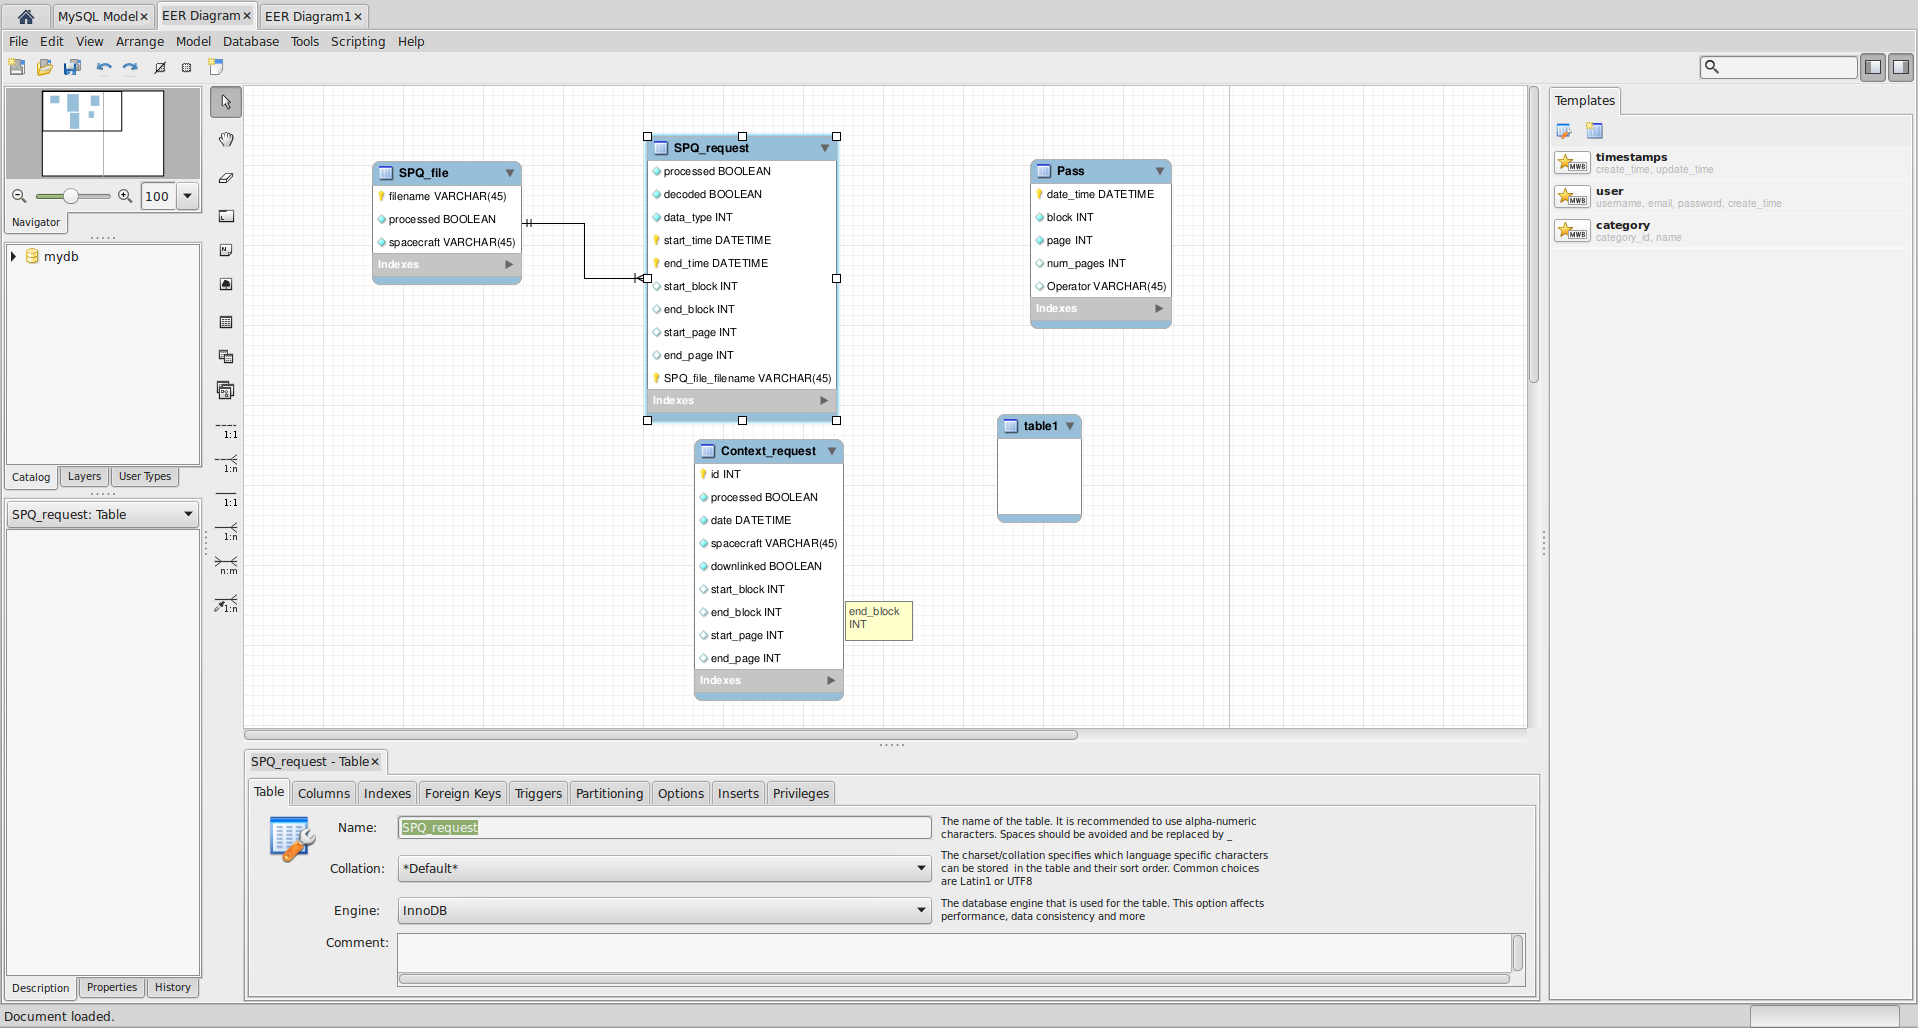
\includegraphics{images/workbench}}  \\
\footnotesize{MySQL Workbench screenshot of incomplete database}

}



\headerbox{First Draft}{name=arch,column=0,span=3, below=abstract}{
\begin{tabular}{ll}
	\begin{minipage}{0.85\columnwidth}
      \resizebox{\columnwidth}{!}{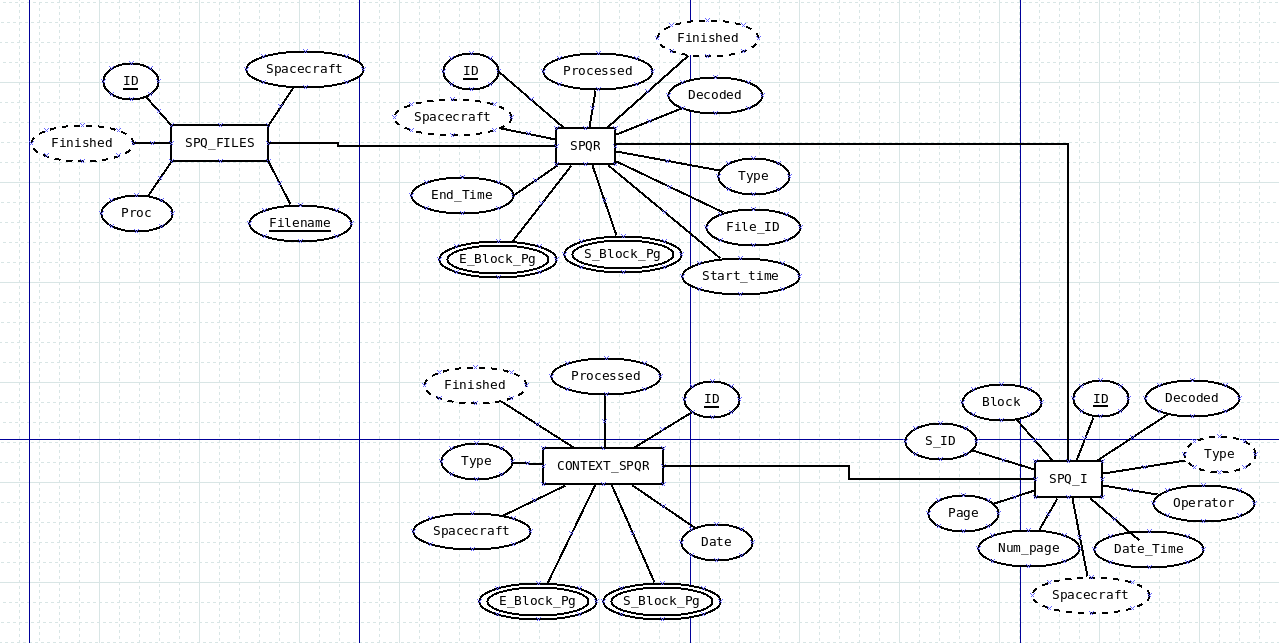
\includegraphics{images/SPQ_Database_ER.png}}
      \footnotesize{ER diagram of first draft}  
	\end{minipage}&

  \begin{minipage}{0.11\columnwidth}
  	\raggedright
     For the first attempt an ER diagram was constructed to visualize the database. Each box indicates a table and each circle represents an entity. The connections define how each table is related. The database was then translated by hand into a MYSQL database. This approach was good for creating a test database but more complex tools were needed to design a more robust database.

  \end{minipage}
    
\end{tabular}
}

\headerbox{Future Work}{name=gloss,column=3,below=hardware}{ 

%\begin{itemize} \itemsep1pt \parskip0pt \parsep0pt \itemindent=-0.5cm
\begin{itemize}[leftmargin=*, noitemsep]
	\item Load data base onto servers.
	\item Write a script that interfaces the database with the ground station
	\item Configure the ground station and database so that down linking of data is automated.
\end{itemize}
\resizebox{\columnwidth}{!}{\includegraphics{images/groundstation}}  \\
\footnotesize{SSEL ground station}
}


\headerbox{Acknowledgment}{name=ack,column=3,below=gloss}{ \footnotesize

\begin{minipage}{\columnwidth}
This work is supported by the NASA Sounding Rocket Program, Grant NNX14AK71G.
 
\end{minipage}
\normalsize
}


\headerbox{References}{name=refs,column=3,below=ack,above=bottom}{\footnotesize
\begin{minipage}{\columnwidth}
[0] Background courtesy of NASA Visible Earth


 
\end{minipage}
\normalsize}

\end{poster}

\end{document}